\documentclass[12pt,aspectratio=169]{beamer}
\usetheme{metropolis}
\setbeamersize{text margin left=.5cm,text margin right=.5cm}
\usepackage[lf]{carlito}
\usepackage{siunitx}
\usepackage{tikz}
\usepackage{mathpazo}
\usepackage{bm}
\usepackage{mathtools}
\usepackage[ISO]{diffcoeff}
\diffdef{}{ op-symbol=\mathsf{d} }
\usepackage{xcolor,colortbl}


\title{Class 20: Circuit Analysis, Part 1}
\subtitle{AP Physics C}
\author[TML]{Dr.\ Timothy Leung}
\institute{Olympiads School}
\date{Updated: Summer 2022}

\newcommand{\pic}[2]{
  \includegraphics[width=#1\textwidth]{#2}
}
\newcommand{\eq}[2]{
  \vspace{#1}{\Large
    \begin{displaymath}
      #2
    \end{displaymath}
  }
}
%\newcommand{\iii}{\ensuremath\hat{\bm{\imath}}}
%\newcommand{\jjj}{\ensuremath\hat{\bm{\jmath}}}
%\newcommand{\kkk}{\ensuremath\hat{\bm{k}}}
%\newcommand{\iii}{\ensuremath\hat x}
%\newcommand{\jjj}{\ensuremath\hat y}
%\newcommand{\kkk}{\ensuremath\hat z}


\begin{document}

\begin{frame}
  \maketitle
\end{frame}




\section{Electric Current}

\begin{frame}{Current}
  The \textbf{electric current} is defined as the rate at which \textbf{charges}
  $Q$ pass through a point in a circuit. In differential form:
  
  \eq{-.1in}{
    \boxed{I(t)=\diff Qt}
%  }
%
%  Expanding the expression:
%
%  \eq{-.1in}{
%    I = \diff Qt
    = \frac QV\diff Vt = (ne)(Av_d)
  }
  \begin{itemize}
  \item $Q/V$ is the amount of charge carriers \emph{per volume}, which
    is just
    the \textbf{charge carrier density} (number of charge carriers per volume)
    $n$ times the \textbf{elementary charge} $e$
  \item $\diff V/t$ is the rate the volume of charges moves through the
    conductor, give by the wire's cross-section area $A$ times the
    \textbf{drift velocity} $v_d$ of the charge carrier
  \end{itemize}
\end{frame}



%\begin{frame}{Current Through the Conductor}
%  Combining the terms:
%
%  \eq{-.1in}{
%    \boxed{I=\diff Qt=neAv_d}
%  }
%  \begin{center}
%    \begin{tabular}{l|c|c}
%      \rowcolor{pink}
%      \textbf{Quantity} & \textbf{Symbol} & \textbf{SI Unit} \\ \hline
%      Current                               & $I$ & \si\ampere \\
%      Charge carrier density                & $n$ & \si{\per\metre\cubed} \\
%      Elementary charge                     & $e$ & \si\coulomb \\
%      Cross-section area of the conductor   & $A$ & \si{\metre\squared}\\
%      Drift velocity of the charge carriers & $v_d$ & \si{\metre\per\second}
%    \end{tabular}
%  \end{center}
%  The calculation for the charge carrier density $n$ requires some additional
%  thoughts.
%\end{frame}



\begin{frame}{Charge Carrier Density}
  Calculating the charge carrier density in a \emph{metal} conductor involves
  some physical information about the metal:
  \begin{enumerate}
  \item Divide the metal's density $\rho$ by its molar mass $M$ to find the
    \emph{number of moles of atoms per unit volume}
  \item Multiply by Avogadro's number $N_A=\SI{6.0221e23}{\per\mol}$ to find
    \emph{number of atoms per unit volume}
  \item Multiply by the number of free electrons per atom $k$ for that
    particular metal
  \end{enumerate}
\end{frame}



\begin{frame}{Charge Carrier Density}
  Collecting all the terms from the last slide, we have:
  
  \eq{-.1in}{
    \boxed{n=\frac{\rho kN_A}M}
  }
  \begin{center}
    \begin{tabular}{l|c|c}
      \rowcolor{pink}
      \textbf{Quantity} & \textbf{Symbol} & \textbf{SI Unit} \\ \hline
      Charge carrier density   & $n$    & \si{\per\metre\cubed} \\
      Density of material      & $\rho$ & \si{\kilo\gram\per\metre\cubed} \\
      Free electrons per atom  & $k$    & \\
      Avogadro's number        & $N_A$  & \si{\per\mol}\\
      Molar mass               & $M$    & \si{\kilo\gram\per\mol}
    \end{tabular}
  \end{center}
  For copper, $M=\SI{63.54e-3}{\kilo\gram\per\mol}$,
  $\rho=\SI{8.96e3}{\kilo\gram\per\metre\cubed}$, $k=1$ and therefore
  $n=\SI{8.5e28}{\per\metre\cubed}$. The drift velocity is in the order of
  $v\approx\SI1{\milli\metre\per\second}$.
\end{frame}



\begin{frame}{Current}
  Another alternate description of the electric current is to express it in
  terms of the \textbf{current density} $J$, with a unit of of \emph{amp\`{e}re
    per meters squared} (\si{\ampere\per\meter\squared}).\footnote{We had
    previously encountered this quantity when studying Amp\`{e}re's law.}

  \eq{-.1in}{
    \boxed{I(t)=J(t)A}
  }

  It is obvious from the previous expression that the current density is the
  product of the charge carrier density, elementary charge, and the drift
  velocity:

  \eq{-.1in}{
    \boxed{J=nev_d}
  }
\end{frame}



\begin{frame}{Electric Current: Conventional vs.\ Electron Flow}
  The flow of electric current assumes the flow of \emph{positive} charges. We
  call this the \textbf{conventional current}:
  \begin{center}
    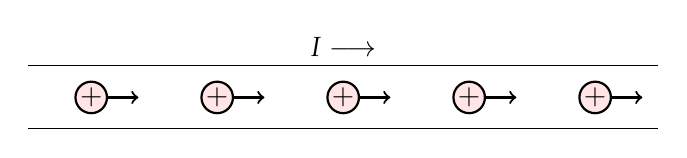
\begin{tikzpicture}[scale=.8]
      \draw (0,0)--(10,0);
      \draw (0,1)--(10,1) node[midway,above]{$I\longrightarrow$};
      \foreach \x in {1,3,...,9}{
        \draw[thick,fill=pink!40](\x,.5) circle(.25) node{$+$};
        \draw[thick,->](\x+.25,.5)--(\x+.75,.5);
      }
    \end{tikzpicture}
  \end{center}
  In a conducting wire, however, negatively charged electrons flow in the
  opposite direction. We call this the \textbf{electron current}:
  \begin{center}
    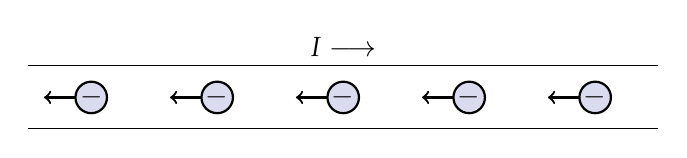
\begin{tikzpicture}[scale=.8]
      \draw (0,0)--(10,0);
      \draw (0,1)--(10,1) node[midway,above]{$I\longrightarrow$};
      \foreach \x in {1,3,...,9}{
        \draw[thick,fill=blue!40!gray!20](\x,.5) circle(.25) node{$-$};
        \draw[thick,->](\x-.25,.5)--(\x-.75,.5);
      }
    \end{tikzpicture}
  \end{center}
  %Even though it is actually electron that are moving, we will continue to
  %treat electric current as the flow of positive charges in the direction of
  %the conventional current.
\end{frame}



\section{Resistors}

\begin{frame}{Resistivity and Electric Field}
  The resistivity of a material is proportional to the electric field and
  current density:

  \eq{-.1in}{
    \boxed{\vec E=\rho\vec J}
    \quad\text{or}\quad
    \boxed{\rho=\left|\frac EJ\right|}
  }
  \begin{center}
    \begin{tabular}{l|c|c}
      \rowcolor{pink}
      \textbf{Quantity} & \textbf{Symbol} & \textbf{SI Unit} \\ \hline
      Electric field & $\vec E$ & \si{\newton\per\coulomb} \\
      Current density & $\vec J$ & \si{\ampere\per\metre\squared} \\
      Resistivity & $\rho$ & \si{\ohm\metre}
    \end{tabular}
  \end{center}
  \begin{itemize}
  \item In a conductor, the electrons are free to move, and the electric
    field tend to be weak, and the resistivity is low.
  \item In an insulator, electrons cannot move easily, therefore the electric
    field are generally strong, and the resistivity is high.
  \end{itemize}
\end{frame}



\begin{frame}{Resistance of a Conductor}
  The resistance of a conductor is proportional to the resistivity $\rho$ and
  its length $L$, and inversely proportional to the cross-sectional area $A$:

  \eq{-.1in}{
    \boxed{
      R=\int\dl R=\rho\int_0^L\frac{\dl x}{A(x)}
    }
  }
  \begin{center}
    \begin{tabular}{l|c|c}
      \rowcolor{pink}
      \textbf{Quantity} & \textbf{Symbol} & \textbf{SI Unit} \\ \hline
      Resistance           & $R$    & \si\ohm \\
      Resistivity          & $\rho$ & \si{\ohm\metre} \\
      Length of conductor  & $L$    & \si\metre \\
      Cross-sectional area & $A(x)$ & \si{\metre\squared}
    \end{tabular}
  \end{center}
\end{frame}


\begin{frame}{Resistance of a Conductor}
  \eq{-.01in}{
    \boxed{R = \rho\frac LA}
  }
  
  \begin{columns}[t]
    \column{.5\textwidth}
    \centering
    \begin{tabular}{c|c|c}
      \rowcolor{cyan}
      {\color{white}Gauge} & 
      {\color{white}Diameter} & 
      {\color{white}$R/L$} \\
      \rowcolor{cyan}
      & {\color{white}(\si{mm})} & 
      {\color{white}(\SI{e-3}{\ohm\per\metre})}\\ \hline
      0  & \num{9.35} & \num{0.31} \\
      10 & \num{2.59} & \num{2.20} \\
      14 & \num{1.63} & \num{8.54} \\
      18 & \num{1.02} & \num{21.90} \\
      22 & \num{0.64} & \num{51.70}
    \end{tabular}
    
    \column{.5\textwidth}
    \centering
    \begin{tabular}{c|c}
      \rowcolor{cyan}
      {\color{white} Material} & 
      {\color{white} Resistivity $\rho$ (\si{\ohm.\metre})}\\ \hline
      silver    & \num{1.6e-8} \\
      copper    & \num{1.7e-8} \\
      aluminum  & \num{2.7e-8} \\
      tungsten  & \num{5.6e-8} \\
      Nichrome  & \num{100e-8} \\
      carbon    & \num{3500e-8}\\
      germanium & \num{.46} \\
      glass     & \num{e10} to \num{e14}
    \end{tabular}
  \end{columns}
\end{frame}




\section{Ohm's Law}

\begin{frame}{Ohm's Law}
  The electric potential difference $V$ across a ``load'' (resistor) equals the
  product of the current $I$ through the load and the resistance $R$ of the
  load.

  \eq{-.1in}{
    \boxed{V=IR}
  }
  \begin{center}
    \begin{tabular}{l|c|c}
      \rowcolor{pink}
      \textbf{Quantity} & \textbf{Symbol} & \textbf{SI Unit} \\ \hline
      Potential difference & $V$    & \si\volt \\
      Current              & $I$    & \si\ampere \\
      Resistance           & $R$    & \si\ohm
    \end{tabular}
  \end{center}
  A resistor is considered ``ohmic'' if it obeys Ohm's law. Note that Ohm's law
  is not a fundamental law in physics.
\end{frame}



\begin{frame}{Ohmic Devices}
  In an ohmic device such as a resistor, the relationship between voltage
  across the device and the current through the device is linear, i.e.:
  \begin{center}
    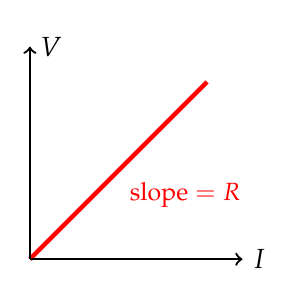
\begin{tikzpicture}[scale=.9]
      \draw[ultra thick,red](0,0)--(2.5,2.5)
      node[midway,below right]{\small $\text{slope}=R$};
      \draw[thick,->](0,0)--(3,0) node[right]{$I$};
      \draw[thick,->](0,0)--(0,3) node[right]{$V$};
    \end{tikzpicture}
    \hspace{.15in}
    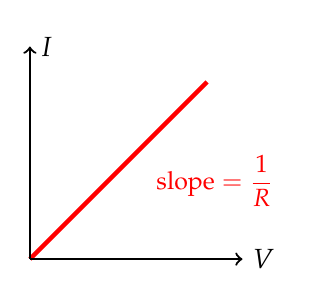
\begin{tikzpicture}[scale=.9]
      \draw[ultra thick,red](0,0)--(2.5,2.5)
      node[pos=.65,below right]{\small $\text{slope}=\dfrac1R$};
      \draw[thick,->](0,0)--(3,0) node[right]{$V$};
      \draw[thick,->](0,0)--(0,3) node[right]{$I$};
    \end{tikzpicture}
  \end{center}
\end{frame}



\begin{frame}{Non-Ohmic Devices}
  Loads that are \textbf{non-ohmic} do not obey Ohm's law: the relationship
  between voltage and current is \emph{not} linear.
  \begin{center}
    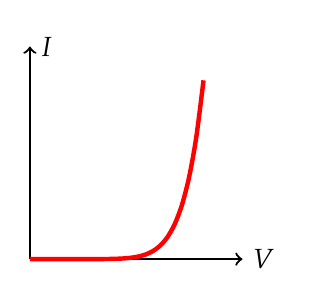
\begin{tikzpicture}[scale=.9]
      \draw[thick,->](0,0)--(3,0) node[right]{$V$};
      \draw[thick,->](0,0)--(0,3) node[right]{$I$};
      \draw[ultra thick,red,domain=0:2.45,smooth] plot(\x,.0008*\x^9);
    \end{tikzpicture}
  \end{center}
  For example, diodes (e.g.\ your TV's LED screen) are non-ohmic.
\end{frame}



\begin{frame}{Power Dissipated by a Resistor}
  Power is the rate at which work $W$ is done, and from electrostatics, the
  change in electric potential energy $\Delta E_q$ is proportional to the
  amount of charge $q$ and the voltage $V$. This gives a very simple expression
  for power through a resistor:
  
  \eq{-.1in}{
    P=\diff Wt=\diff {E_q}t=\diff{(qV)}t=\left(\diff qt\right)V
    \;\rightarrow\;\boxed{P=IV}
  }

  Combining Ohm's law with the above equation gives two additional expressions
  for power through a resistor:

  \eq{-.1in}{
    \boxed{P=\frac{V^2}R}\quad\quad\boxed{P=I^2R}
  }
\end{frame}


\section{Kirchhoff's Laws}

\begin{frame}{Kirchhoff's Current Law}
  The electric current that flows into any junction in an electric circuit must
  be equal to the current which flows out.

  \vspace{.2in}
  \begin{columns}
    \column{.4\textwidth}
    \begin{tikzpicture}[scale=1.6]
      \begin{scope}[thick]
        \draw(.2,1) to[short,o-] (1.5,1)--(3.5,1)--(3.5,-.2);
        \draw(1.5,1)--(1.5,-.2);
        \draw(2.5,1)--(2.5,-.2);
      \end{scope}
      \begin{scope}[ultra thick,->,red]
        \foreach\x in {1,...,3}{
          \draw(\x+.5,.9)--(\x+.5,.1)   node[midway,left]{$I_{\x}$};
        }
        \draw(.4,1)--(1.3,1) node[midway,above]{$I$};
      \end{scope}
    \end{tikzpicture}

    \column{.6\textwidth}
    In the example on the left, with $I$ going into the junction, and $I_1$,
    $I_2$ and $I_4$ coming out, the current law says that

    \eq{-.1in}{
      I=I_1+I_2+I_3
    }

    Basically, it means that there cannot be any accumulation of charges
    anywhere in the circuit. The law is a consequence of conservation of charge.
  \end{columns}
\end{frame}



\begin{frame}{Kirchhoff's Voltage Law}
  The voltage changes around any closed loop in the circuit must sum to zero,
  no matter what path you take through an electric circuit.

  \vspace{.1in}
  \begin{columns}
    \column{.3\textwidth}
    \begin{center}
      \begin{tikzpicture}[scale=1.8,american voltages]
        \draw[thick](0,0) to[battery1,l=$\mathcal E$] (0,1.5)--(1.2,1.5)
        to[R=$R$] (1.2,0)--(0,0);
      \end{tikzpicture}
    \end{center}
    \column{.7\textwidth}
    Assume that the current flows clockwise and we draw a clockwise loop, we
    get

    \eq{-.1in}{
      \mathcal E-V_R=0\;\;\rightarrow\;\; \mathcal E-IR=0
    }
  \end{columns}
\end{frame}



\section{Resistors in Circuits}

\begin{frame}{Resistors in Parallel}
  \begin{columns}
    \column{.32\textwidth}
    \begin{tikzpicture}
     \draw[thick](0,2) to[short,o-] (1,2)to[R=$R_1$] (1,0) to[short,-o] (0,0);
     \draw[thick](1,2) to[short] (2.25,2)to[R=$R_2$] (2.25,0)to[short] (1,0);
     \draw[thick](2.25,2)to[short](3.5,2) to[R=$R_3\cdots$] (3.5,0)
     to[short] (2.25,0);
    \end{tikzpicture}
    
    \column{.68\textwidth}
    The total current is the current through all the resistors, which can be
    rewritten in terms of voltage and resistance using Ohm's law:

    \eq{-.1in}{
      I=I_1+I_2+I_3\cdots=\frac{V_1}{R_1}+\frac{V_2}{R_2}+\frac{V_3}{R_3}\cdots
    }
    
    Since $V_1=V_2=V_3=\cdots=V$ from the voltage law, we can re-write as

    \eq{-.1in}{
      I=\frac V{R_p}=V\left(\frac1{R_1}+\frac1{R_2}+\frac1{R_3}
      \cdots\right)
    }
  \end{columns}
\end{frame}



\begin{frame}{Equivalent Resistance of Resistors in Parallel} 
  The reciprocal of the equivalent resistance for resistors connected in
  parallel is the sum of the inverses of the individual resistances.

  \eq{-.1in}{
    \boxed{
      \frac1{R_p}=\sum_i^N\frac1{R_i}
    }
  }
  \begin{center}
    \begin{tabular}{l|c|c}
      \rowcolor{pink}
      \textbf{Quantity} & \textbf{Symbol} & \textbf{SI Unit} \\ \hline
      Equivalent resistance in parallel & $R_p$ & \si\ohm \\
      Resistance of individual loads    & $R_i$ & \si\ohm
    \end{tabular}
  \end{center}
  Connecting resistors in parallel effetively increases the cross-sectional
  area, and therefore decreases equivalent resistance.
\end{frame}



\begin{frame}{Resistors in Series}
  \begin{center}
    \begin{tikzpicture}
      \draw[thick](0,0) to[R=$R_1$,o-] (2,0) to[R=$R_2$] (4,0)
      to[R=$R_3$,-o] (6,0);
    \end{tikzpicture}
  \end{center}

  \vspace{.1in}The analysis for resistors in series is similar (but easier).
  From the current law, the current through each resistor is the same:

  \eq{-.1in}{I_1=I_2=I_3=\cdots=I}

  \vspace{-.15in}And the total voltage drop across all resistor is therefore:

  \eq{-.1in}{
    V=V_1+V_2+V_3+\cdots=I(R_1+R_2+R_3+\cdots)
  }
\end{frame}



\begin{frame}{Equivalent Resistance: Resistors in Series}
  The equivalent resistance of loads is the sum of the resistances of the
  individual loads.
  
  \eq{-.1in}{
    \boxed{R_s=\sum_{i=1}^NR_i}
  }
  \begin{center}
    \begin{tabular}{l|c|c}
      \rowcolor{pink}
      \textbf{Quantity} & \textbf{Symbol} & \textbf{SI Unit} \\ \hline
      Equivalent resistance in series & $R_s$ & \si\ohm \\
      Resistance of individual loads  & $R_i$ & \si\ohm
    \end{tabular}
  \end{center}
  Connecting resistors in series effetively increases the length, and
  therefore increases equivalent resistance.
\end{frame}


%\begin{frame}{Example Problem (Simple)}
%  A simple circuit analysis problem will involve one voltage source and
%  resistors connected, some in parallel, and some in series. Below is a typical
%  example:
%
%  \vspace{.2in}
%  \begin{columns}
%    \column{.4\textwidth}
%    \begin{tikzpicture}[scale=.8,american voltages]
%      \draw(0,0) to[R=2<\ohm>](0,2) to[battery=100<\volt>] (0,4) to[short]
%      (1,4) to [R=10<\ohm>] (3,4)--(3,4.5) to[R=40<\ohm>] (5,4.5)
%      to[short] (5,4) to[short] (5.5,4)--(5.5,0)--(0,0);
%      \draw(3,4)--(3,3.5) to[R,l_=10<\ohm>] (5,3.5)--(5,4);
%      \draw[dashed] (-1.8,0.25) rectangle(0.6,3.75);
%    \end{tikzpicture}
%    \column{.6\textwidth}
%    Two \SI{10}{\ohm} resistors and a \SI{40}{\ohm} resistor are connected as
%    shown to a \SI{100}{\volt} emf source with internal resistance
%    \SI{2}{\ohm}. How much power is dissipated by the \SI{40}{\ohm} resistor?
%    \begin{enumerate}[(A)]
%    \item\SI{160}{\watt}
%    \item\SI{40}{\watt}
%    \item\SI{400}{\watt}
%    \item\SI{5}{\watt}
%    \item\SI{500}{\watt}
%    \end{enumerate}
%  \end{columns}
%\end{frame}



\begin{frame}{Tips for Solving ``Simple'' Circuit Problems}
  \begin{enumerate}
  \item Identify groups of resistors that are in parallel or in series, and
    find their equivalent resistance.
  \item Gradually reduce the entire circuit to one voltage source and one
    resistor.
  \item Using Ohm's law, find the current out of the battery.
  \item Using Kirchhoff's laws, find the current through each of the resistors.
  \end{enumerate}
\end{frame}




\section{Multi-loop Circuit}

\begin{frame}{Circuits Aren't Always Simple}
  Some of these problems require you to solve a system of linear equations.
  The following is a simple example with two voltage sources:
  \begin{center}
    \begin{tikzpicture}[american voltages,scale=1.3]
      \draw[thick](0,0) to[battery,l=$\mathcal E_1$](0,2) to[R,l=$R_1$](2,2)
      to[R,l=$R_3$](2,0)--(0,0);
      \draw[thick](2,0)--(4,0) to[battery,l_=$\mathcal E_2$](4,2)
      to[R,l_=$R_2$](2,2);
      \uncover<2->{
        \draw[very thick,red,->](2,0.4)--(2,0)
        node[midway,right]{\small $I_1+I_2$};
        \draw[very thick,red,->] (0.6,0.4)..controls (0,2) and (2,2)..(1.6,.4)
        node[midway,below]{\small $I_1$};
        \draw[very thick,red,->] (3.4,0.4)..controls (4,2) and (2,2)..(2.4,.4)
        node[midway,below]{\small $I_2$};
      }
    \end{tikzpicture}
  \end{center}
  \uncover<2->{
    In this case, we have to draw two loops of current.
  }
\end{frame}



%\begin{frame}{A More Difficult Example}
%  \begin{columns}
%    \column{.4\textwidth}
%    
%    \vspace{-.3in}
%    \begin{tikzpicture}[american voltages]
%      \draw(0,0) to[battery=$V_1$](0,2) to[R=$R_1$](2,2)to[R=$R_3$](2,0)--(0,0);
%      \draw(2,0)--(4,0) to[battery,l_=$V_2$](4,2) to[R,l_=$R_2$](2,2);
%      \draw[very thick,red,->](2,0.4)--(2,0)
%      node[midway,right]{\tiny $I_1+I_2$};
%      \draw[very thick,red,->] (0.6,0.4)..controls (0,2) and (2,2)..(1.6,.4)
%      node[midway,below]{\tiny $I_1$};
%      \draw[very thick,red,->] (3.4,0.4)..controls (4,2) and (2,2)..(2.4,.4)
%      node[midway,below]{\tiny $I_2$};
%    \end{tikzpicture}
%    \column{.6\textwidth}
%    We split the circuit into two loops, and apply Kirchkoff's voltage in both:
%
%    \vspace{-.4in}{\Large
%      \begin{align*}
%        V_1-I_1R_1-(I_1+I_2)R_3&=0\\
%        V_2-I_2R_2-(I_1+I_2)R_3&=0
%      \end{align*}
%    }
%  \end{columns}
%
%  \vspace{-.1in}Two equations, two unknowns ($I_1$ and $I_2$). We can subtract
%  (2) from (1), then solve for $I_1$ and $I_2$:
%
%  \eq{-.4in}{
%    I_1=\frac{V_1-I_2R_3}{R_1+R_3}
%    \quad\quad
%    I_2=
%    \frac{\left[V_2-\frac{(V_1-V_2)R_3}{R_1}\right]}
%         {\left[R_2+\frac{(R_1+R_2)R_3}{R_1}\right]}
%  }
%
%  (Try this at home as an exercise.)
%\end{frame}


\begin{frame}{As Difficult As It Gets}
  \begin{columns}
    \column{.45\textwidth}
    \begin{tikzpicture}[american voltages,scale=1.2]
      \draw[thick](0,0)--(0,2) to[R=3<\ohm>] (0,4)
      to[battery1,l=42<\volt>] (2,4) to[R=3<\ohm>] (4,4)--(4,2)
      to[R=4<\ohm>](4,0)--(2,0) to[battery1,l=6<\volt>] (2,2)
      to[R,l_=4<\ohm>] (0,2);
      \draw[thick](0,0) to[R,l_=6<\ohm>](2,0);
      \draw[thick](2,2) to[R,l_=6<\ohm>](4,2);
      \uncover<2->{
        \begin{scope}[ultra thick, red,->]
          \draw (.5,3.5)..controls(4.75,4)and(4.75,2)..(.5,2.5)
          node[midway,left]{$I_1$};
          \draw (0.6,0.4)..controls (0,2) and (2,2)..(1.4,.4)
          node[midway,below]{$I_3$};
          \draw (2.6,0.4)..controls (2,2) and (4,2)..(3.4,.4)
          node[midway,below]{$I_2$};
        \end{scope}
      }
    \end{tikzpicture}
    
    \column{.55\textwidth}
    \begin{itemize}
    \item To solve this problem, we define a few ``loops'' around the circuit:
      one on top, one on bottom left, and one on bottom right.
    \item<2-> Apply the voltage law in the loops. For example, in the
      lower left:

      \eq{-.1in}{
        4(I_1-I_3)-6-6I_3=0
      }      
    \item<2-> Solve the linear system to find the current. If the current that
      you worked out is negative, it means that you have the direction wrong.
    \end{itemize}
  \end{columns}
\end{frame}
\end{document}
